\documentclass{article}
\usepackage{graphicx}
\usepackage[affil-it]{authblk}
\usepackage{url}
\usepackage{nth}
\usepackage{float}
\usepackage{multirow}

\begin{document}

\title{Developing a driver for a film scanner by means of USB sniffing and reverse engineering}
\author{Hugo Platzer \\ University of Salzburg}
\maketitle

\section{The USB standard}

\subsection{Motivation}

USB is an interface intended to connect various peripherals to PCs. These include:
Human interface devices like keyboards and mice; storage devices like card readers,
external hard disks, memory sticks and smartphones; multimedia devices like microphones, speakers,
cameras and scanners. Some highlights leading to its wide adoption \cite[p. 11]{usbstd}:

\begin{itemize}
  \item Unified interface for all kinds of peripherals
  \item Plug and play: The user plugs in the device, the configuration (e.g. loading the appropriate drivers)
  is done automatically by the operating system
  \item Number of ports can be increased using hubs. Multiple hubs can be chained
        allowing for up to 127 devices on a single root port.
  \item High data rate of 480 Mbit / s (USB 2.0 high-speed mode). Also offers low-latency
        transfers for real-time audio/video applications
  \item Backwards compatibility: Older USB 1.1 devices can be used at 2.0 hosts.
        High-speed USB 2.0 devices can also be used on older
        machines supporting only USB 1.1 (albeit at lower speed).
\end{itemize}

\subsection{Electrical side}

\begin{figure}[!htbp]
  \caption{USB cable cross-section \cite[p. 17]{usbstd}}
  \centering
  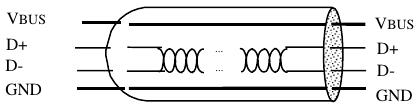
\includegraphics[width=0.5\textwidth]{images/usb_cable.jpg}
\end{figure}

A USB cable has four wires: One as ground, VBUS for a 5 V power supply and two for data transmission.
The power line allows it to draw up to 100 mA without any configuration. This is useful for simple
devices that are not using the data lanes, just the power, like USB lights. Also it allows for devices
not taking much power to be self-powered which eliminates the need for an extra power supply and connector.
Devices can ask the host for more power (up to 500 mA), those that need even more (like a lot of scanners) need
an external supply. \cite[p. 17f.]{usbstd}

\subsection{Signaling}

\subsubsection{Low-level states}

USB is a serial bus which means there is only a single path for data transmission.
Differential signalling across the D- and D+ wires is used, which means the difference in voltage
across the two wires (rather than some absolute) determines the state. This is beneficial because
noise during transmission should affect both lines equally, not changing the difference.
Higher frequencies and thus data rates become possible.

\begin{table}[!htbp]
  \caption{USB speed modes \cite[p. 159]{usbstd}}
  \centering
  \begin{tabular}{l | l | l}
    Mode & Speed & Bit time \\ \hline
    Low Speed & 1.5 Mbit / s & 667 ns \\
    Full Speed & 12 Mbit / s & 83 ns \\
    High Speed & 480 Mbit / s & 2 ns \\
  \end{tabular}
\end{table}

\begin{table}[!htbp]
  \caption{Low-level data line states (only applies to Full Speed) \cite[p. 145]{usbstd}}
  \centering
  \begin{tabular}{l | l}
    Levels & State \\ \hline
    Differential '0' & D- high, D+ low \\
    Differential '1' & D- low, D+ high \\
    Single Ended Zero (SE0) & both low \\
    Single Ended One (SE1) & both high (illegal state, should never happen) \\
    Data 'J' state & Differential '1' \\
    Data 'K' state & Differential '0' \\
    Idle state & Data 'J' state \\
    Start of Packet (SOP) & Switch from idle to 'K' \\
    End of Packet (EOP) & SE0 for 2 bit times followed by 'J' for 1 bit time \\
    Disconnect & SE0 for $\geq$ 2 us \\
    Connect & Idle for 2.5 us \\
    Reset & SE0 for $\geq$ 2.5 us \\
  \end{tabular}
\end{table}

\pagebreak
Low Speed is used for devices where speed is not important (mice, keyboards).
It allows for cheaper cables and electronics. High Speed is only available
in USB 2.0. For reasons of simplicity, only full speed signaling will be covered
here. \cite[p. 12]{usbstd}

SE0 is the state of the data lines if no device is connected. The host
recognizes a device being plugged in by the D+ line being "pulled up" to high.
It then most likely initiates a reset so the device is in a known state for
communication to begin. Similarly, a disconnect is sensed by a SE0 for some time.
\cite[p. 149]{usbstd}

It is important to note that {\bf all communication on the USB bus is initiated by the
host}. Devices on the bus can not directly talk to each other and can only talk
to the host as a direct response to a request made by it before.
\cite[p. 27]{usbstd}

\subsubsection{Bitstream encoding}

USB uses NRZI encoding for the transmitted data: A zero is represented by a change to
the opposite state while a one is represented by staying in the same state.

\begin{figure}[!htbp]
  \caption{NRZI bitstream encoding \cite[p. 157]{usbstd}}
  \centering
  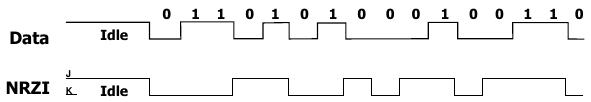
\includegraphics[width=0.5\textwidth]{images/nrzi_encoding.jpg}
\end{figure}

For keeping the receiver clock in sync with the data it is not ideal if the signal
stays at J or K for too long. To prevent this, a technique called "bit stuffing"
is used: Before doing NRZI encoding, a zero is inserted after every six consecutive ones
in the data. The receiver recognizes the stuffed bits during decoding and discards them.
\cite[p. 157]{usbstd}

\subsection {Packets}

Packets are the atomic unit of data transmission in USB. In between packet transmission,
the bus remains in an idle state. Every packet starts with a sync pattern to synchronize
the clocks between sender and receiver. Next are the actual data bits. The packet is
terminated by an EOP state. Fields in a packet are transmitted least-significant
bit first. \cite[p. 195]{usbstd}

The first 8 bits of every packet contain the packet ID (PID) which identifies its type
and thus how the rest of the packet data should be interpreted. The PID is 4 bits long, they are transmitted a second time in reverse bit order to allow the receiver to quickly
discard a faulty packet. There are 17 different packet types (PRE and ERR have the same ID,
some are only relevant for High Speed) \cite[p. 195]{usbstd}:

\begin{table}[!htbp]
  \caption{USB packet types; notice how the least-significant two bits identify the packet category \cite[p. 196]{usbstd}}
  \centering
  \begin{tabular}{l | l | l | p{5cm}}
    PID type & PID name & \begin{tabular}{@{}l} PID bits \\ (3..0) \end{tabular} & Description \\ \hline
    \multirow{4}*{Token} & OUT & 0001 & Address + endpoint number for host-to-device transaction \\
                         & IN & 1001 & Address + endpoint number for device-to-host transaction \\
                         & SOF & 0101 & Start-of-frame marker, frame number \\
                         & SETUP & 1101 & Special host-to-device transaction for device configuration \\ \hline
    \multirow{4}*{Data} & DATA0 & 0011 & Data packet \\
                         & DATA1 & 1011 & Data packet \\
                         & DATA2 & 0111 & Data packet (only High Speed) \\
                         & MDATA & 1111 & Data packet (only High Speed) \\ \hline
    \multirow{4}*{Handshake} & ACK & 0010 & Receiver accepts error-free data packet \\
                         & NAK & 1010 & Receiver cannot accept data or transmitter cannot send data \\
                         & STALL & 1110 & Endpoint halted or control pipe request not supported \\
                         & NYET & 0110 & Data packet (only High Speed) \\ \hline
    \multirow{4}*{Special} & PRE & 1100 & Preamble to enable downstream traffic to low-speed devices \\
                         & ERR & 1100 & Split Transaction error handshake \\
                         & SPLIT & 1000 & High speed Split Transaction token (only High Speed) \\
                         & PING & 0100 & High speed control flow probe (only High Speed) \\
                         & Reserved & 0000 & Reserved PID \\
  \end{tabular}
\end{table}

\subsubsection{Token packet}

\begin{figure}[H]
  \caption{Token packet format \cite[p. 199]{usbstd}}
  \centering
  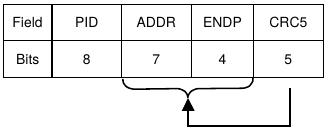
\includegraphics[width=0.5\textwidth]{images/token_packet.jpg}
\end{figure}

Token packets are used at the start of so-called transactions to specify the target
of the transaction on the bus, namely a certain device and endpoint. There are 127
possible devices on a bus (address 0 is reserved for a device that has not been configured yet).
\cite[p. 256]{usbstd}

Endpoints are logical entities on a device that are used as sources and sinks of data
in so-called pipes. A pipe is either in OUT (to device) or IN (to host) direction.
Endpoint 0 is a special bidirectional pipe that must be available on every device
right after the reset. It is used mainly for identifying and configuring the device.
\cite[p. 33]{usbstd}

\subsubsection{Data packet}

\begin{figure}[H]
  \caption{Data packet format \cite[p. 206]{usbstd}}
  \centering
  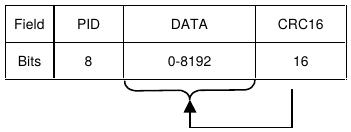
\includegraphics[width=0.5\textwidth]{images/data_packet.jpg}
\end{figure}

Used to transmit the actual data in a transaction.

\subsubsection{Handshake packet}

\begin{figure}[H]
  \caption{Handshake packet format \cite[p. 206]{usbstd}}
  \centering
  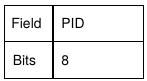
\includegraphics[width=0.21\textwidth]{images/handshake_packet.jpg}
\end{figure}

Used to report the status of a transaction.

\subsection{Transfers}

Transfers are the abstraction level of data exchange as seen at the software
side of the host. From the host's perspective, a transfer transmits a string of
 bytes from / to the device. A transfer is directed to one of the device's endpoints,
each of them has one of four transfer types plus a transfer direction
asscociated with it during device configuration.
Transfers are composed of transactions, which usually consist of three
packets \cite[p. 209ff.]{usbstd}:

\begin{enumerate}
  \item A token packet to tell the type of the transaction and its destination
        (as all USB communication is initiated by the host, the token packet always comes
        from the host)
  \item A DATA packet for the actual payload. Length can vary between 8-64 bytes on Full Speed links.
        This can go host to device or device to host.
  \item A handshake packet (usually ACK, NAK) lets the sender know if the data was received successfully.
\end{enumerate}

Transfers usually consist of multiple transactions.

\begin{figure}[H]
  \caption{Composition of a USB transfer \cite[p. 44]{uc}}
  \centering
  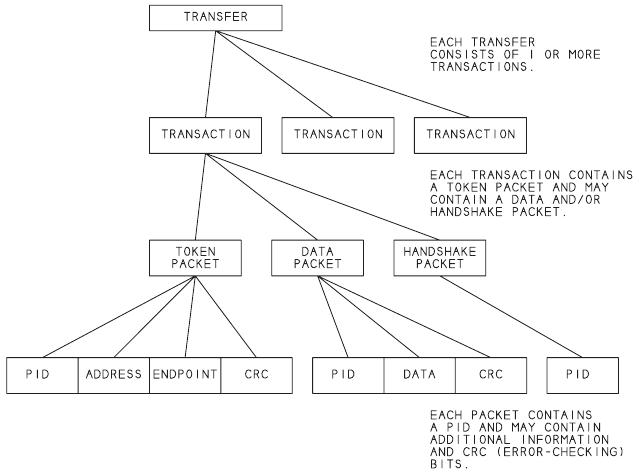
\includegraphics[width=\textwidth]{images/transfer_tree.jpg}
\end{figure}

\subsubsection {Control transfer}

Every device must have endpoint 0 for control transfers. Control endpoints
are message-based. This means each transfer is for a specific message which has
defined length, format and purpose. There can be transfers in either direction
on the same endpoint, although each transfer has a specified (data stage) direction.
Control transfers start with a Setup stage / transaction specifying the target device
and endpoint plus an extra 8 bytes of data called the Device Request. \cite[p. 38f.]{usbstd}

\begin{table}[H]
  \caption{Device Request format \cite[p. 248]{usbstd}}
  \centering
  \begin{tabular}{l | l | l | p{5.5cm}}
    \begin{tabular}{@{}l} Offset \\ (bytes) \end{tabular} & Field &
    \begin{tabular}{@{}l} Size \\ (bytes) \end{tabular} & Description \\ \hline
    
    0 & bmRequestType & 1 &
    
      Bits 0..4: Recipient
      
      \begin{tabular}{l l}
        0 & Device \\
        1 & Interface \\
        2 & Endpoint \\
        3 & Other \\
        4..31 & Reserved \\
      \end{tabular}
      
      \vspace{3mm}
      Bits 5..6: Type
      
      \begin{tabular}{l l}
        0 & Standard \\
        1 & Class \\
        2 & Vendor \\
        3 & Reserved \\
      \end{tabular}
      
      \vspace{3mm}
      Bit 7: Transfer direction
      
      \begin{tabular}{l l}
        0 & Host to device \\
        1 & Device to host \\
      \end{tabular} \\ \hline
  
    1 & bRequest & 1 & Specific request \\ \hline
    2 & wValue & 2 & Varies according to request \\ \hline
    4 & wIndex & 1 & Varies according to request, typically used
    for a index or offset \\ \hline
    6 & wLength & 2 & Number of bytes to be transferred in the data stage
    (0 means no data stage) \\
  \end{tabular}
\end{table}

Depending on the kind of control transfer, there may be a data stage
consisting of data transactions, but this is not required. If there
are data transactions, all are going in the same direction as specified
by the request type.
The transfer is completed with a Status transaction to report back
about the success of the whole transfer.

Control transfers are used right after the device reset to get information about
its capabilities and set a configuration. For this, there are 11 bRequest values
called Standard Requests that have to be supported by all devices as part of the standard.

\begin{table}[H]
  \caption{Some important Standard Requests \cite[p. 250]{usbstd}}
  \centering
  \begin{tabular}{l | l | p{2cm} | p{2cm}}
    bRequest & \begin{tabular}{@{}l}  bmRequestType \\ (7..0) \end{tabular}
     & wValue & wIndex \\ \hline
    
    GET\_DESCRIPTOR & 10000000 & Descriptor type and index & Zero or Language ID \\ \hline
    SET\_ADDRESS & 00000000 & Device address & Zero \\ \hline
    GET\_STATUS & \begin{tabular}{@{}l}  10000000 \\ 10000001 \\ 10000010 \end{tabular}
    & Zero & \begin{tabular}{@{}l}  Zero \\ Interface \\ Endpoint \end{tabular} \\ \hline
    SET\_CONFIGURATION & 00000000 & Configuration value & Zero \\
  \end{tabular}
  
  \vspace{5mm}
  \begin{tabular}{l | l | p{5cm}}
    bRequest & wLength & Data \\ \hline
    
    GET\_DESCRIPTOR & Descriptor length & Descriptor \\
    SET\_ADDRESS & None & None \\
    GET\_STATUS & Two & Device, Interface or endpoint status \\
    SET\_CONFIGURATION & None & None \\
  \end{tabular}
\end{table}

They are also used to control the device after the configuration phase during normal operation.
There are standardized requests (Class Requests) for certain device classes like keyboards, storage devices etc.

Other non-standard devices have custom, vendor-specific requests that are not documented
in the USB standard.

\subsubsection {Bulk transfer}

Bulk transfers are used to transmit large amouts of data with guaranteed delivery
and low overhead but no latency / bandwidth constraints.
Compared to control transfers, they are stream-based. This means there is no defined message
format or size. For an IN endpoint, the host would poll the device endpoint for data until it receives
(cumulative) as many bytes as requested by the software. A transfer can also be ended by the device sending
a data transaction of less size than the maximum of this endpoint (data is always split so there is at most one
smaller packet at the end) or a zero-size data transaction. To avoid data packets being lost, they
alternate between the DATA0 / DATA1 PIDs. A single bulk endpoint is only for incoming
or only for outgoing transfers.
The host schedules them at times when the bus bandwidth is not used by other transfer types.
Typical uses for bulk transfers are transferring data from/to an external harddrive,
to a printer or from a scanner. \cite[p. 52ff.]{usbstd}

\subsubsection {Interrupt transfer}

On the bus, interrupt transfers look the same as bulk transfers.
The main difference is scheduling: The host guarantees that a transfer
attempt is made as often as specified in the endpoint descriptor (1 - 100 ms).
Despite the name, interrupt transfers have nothing to do with hardware interrupts.
All communication on the USB bus is initiated by the host, so it has to poll the device
for data.
Typical uses for interrupt transfers are receiving keypresses from keyboards and
movements from mice. \cite[p. 48ff.]{usbstd}

\subsubsection {Isochronous transfer}

Isochronous transfers are for transmitting data at a constant rate with guaranteed
latency. Compared to interrupt transfers, they offer a guaranteed transfer rate
(with interrupt transfers the interval between two transfers can be anywhere
between zero and the specified maximum). The drawback is a lack of any handshake
/ retry mechanism.
Typical uses for isochronous transfers are USB sound cards or webcams.
\cite[p. 44ff.]{usbstd}

\subsection{Device initialization}

The process from a device being plugged in to it becoming usable for the user
roughly goes as follows (every USB bus has at least a root hub device interacting with
the operating system) \cite[p. 87ff.]{uc}:

\begin{enumerate}
  \item The hub detects the device by the change in levels on the data lines.
  \item The hub reports the device to the host.
  \item The host tells the hub to reset the device so communication can begin.
  \item The host assigns an address to the new device.
  \item The host asks for the Device Descriptor to get information identifying the device
        (vendor / product ID, device class).
  \item The host looks for a driver handling this VID / PID combination, if it does not find one,
        it leaves the device in an unconfigured state.
  \item If a driver is found, it is loaded. The device is asked for its configuration profiles.
        The driver sets a configuration and can now make the device serve its purpose.
\end{enumerate}

\subsubsection{Device descriptor}

After setting the address, a GET\_DESCRIPTOR
device request is made, asking for the device descriptor.

\subsubsection{Configuration descriptor}

\subsubsection{Interface descriptor}

\subsubsection{Endpoint descriptor}

\begin{thebibliography}{}

\bibitem{usbstd}
Universal Serial Bus Specification, Revision 2.0. April 27, 2000. Available at \url{http://www.usb.org/developers/docs/usb20_docs/}

\bibitem{uc}
USB Complete: Everything You Need to Develop Custom USB Peripherals (\nth{3} edition).
Jan Axelson, Lakeview Research LLC 2012. ISBN: {\tt   978-1-931448-03-1}


\end{thebibliography}

\end{document}
